\subsection{Full System Operation}
The result of this finalized implementation was a proof of concept SLAM system capable of generating compass-referenced 2D floorplans of its surroundings, as well as 3D depth maps of its entire field of view. The operating modes of this device were user-selectable, and were output to an external VGA display. The final hardware implementation of the project is shown in Figure \ref{finalHW}. Note that the stereo cameras and digital compass were mounted rigidly to the ZedBoard, while the scanning laser rangefinder and RS232-TTL converter were attached externally.
\par
\begin{figure}[H]
	\centerline{
	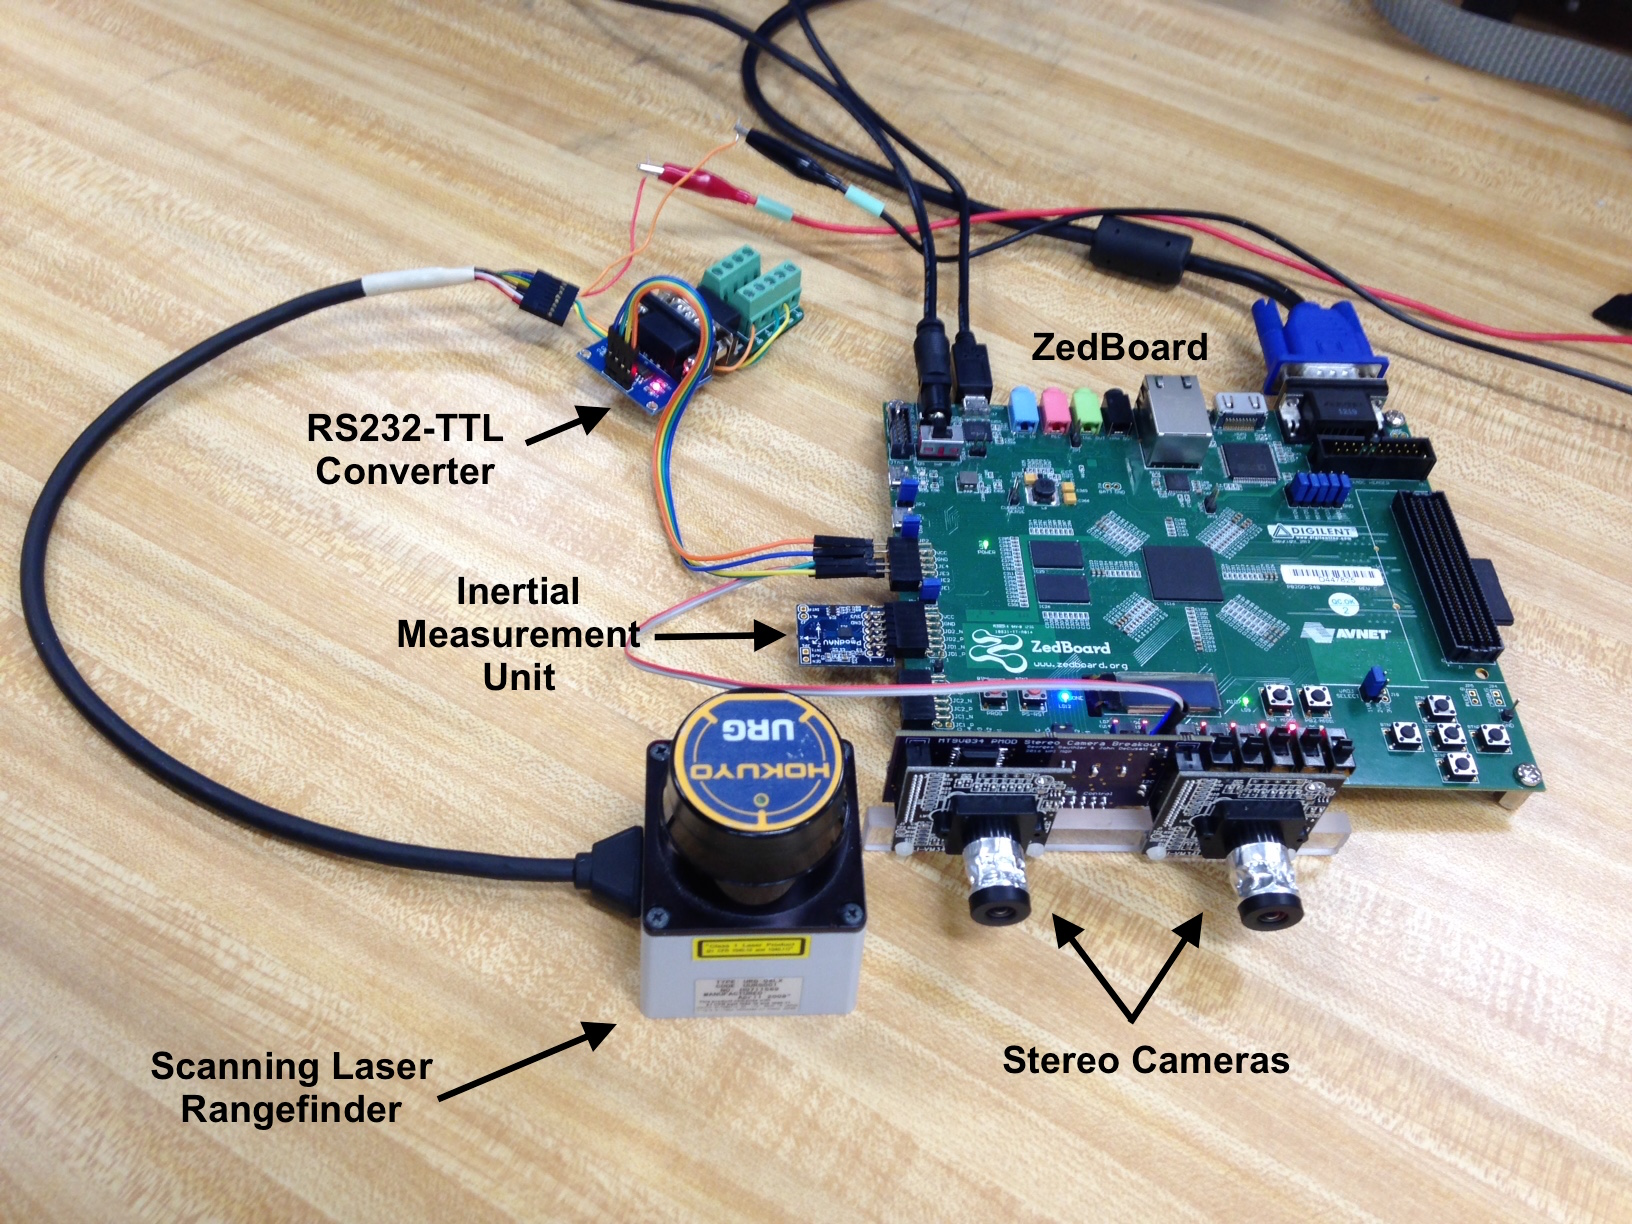
\includegraphics[width=1\linewidth]{setup_label.JPG}
	}
	\caption{System Hardware}
	\label{finalHW}
\end{figure}
\par
An overall system block diagram is shown in Figure \ref{systemBD2}. The system implementation was broken down into several major components. At the top level, the Zynq-7000 ARM Cortex A9 processing system was used for controlling low-level sensor peripherals. These included the stereo camera I$^2$C lines, as well as UART and SPI interfaces for the rangefinder and digital compass, respectively. The ARM processor was also used for continuously pre-parsing rangefinder and digital compass data before it was written to the programmable logic.
\par
\begin{figure}[H]
	\centerline{
	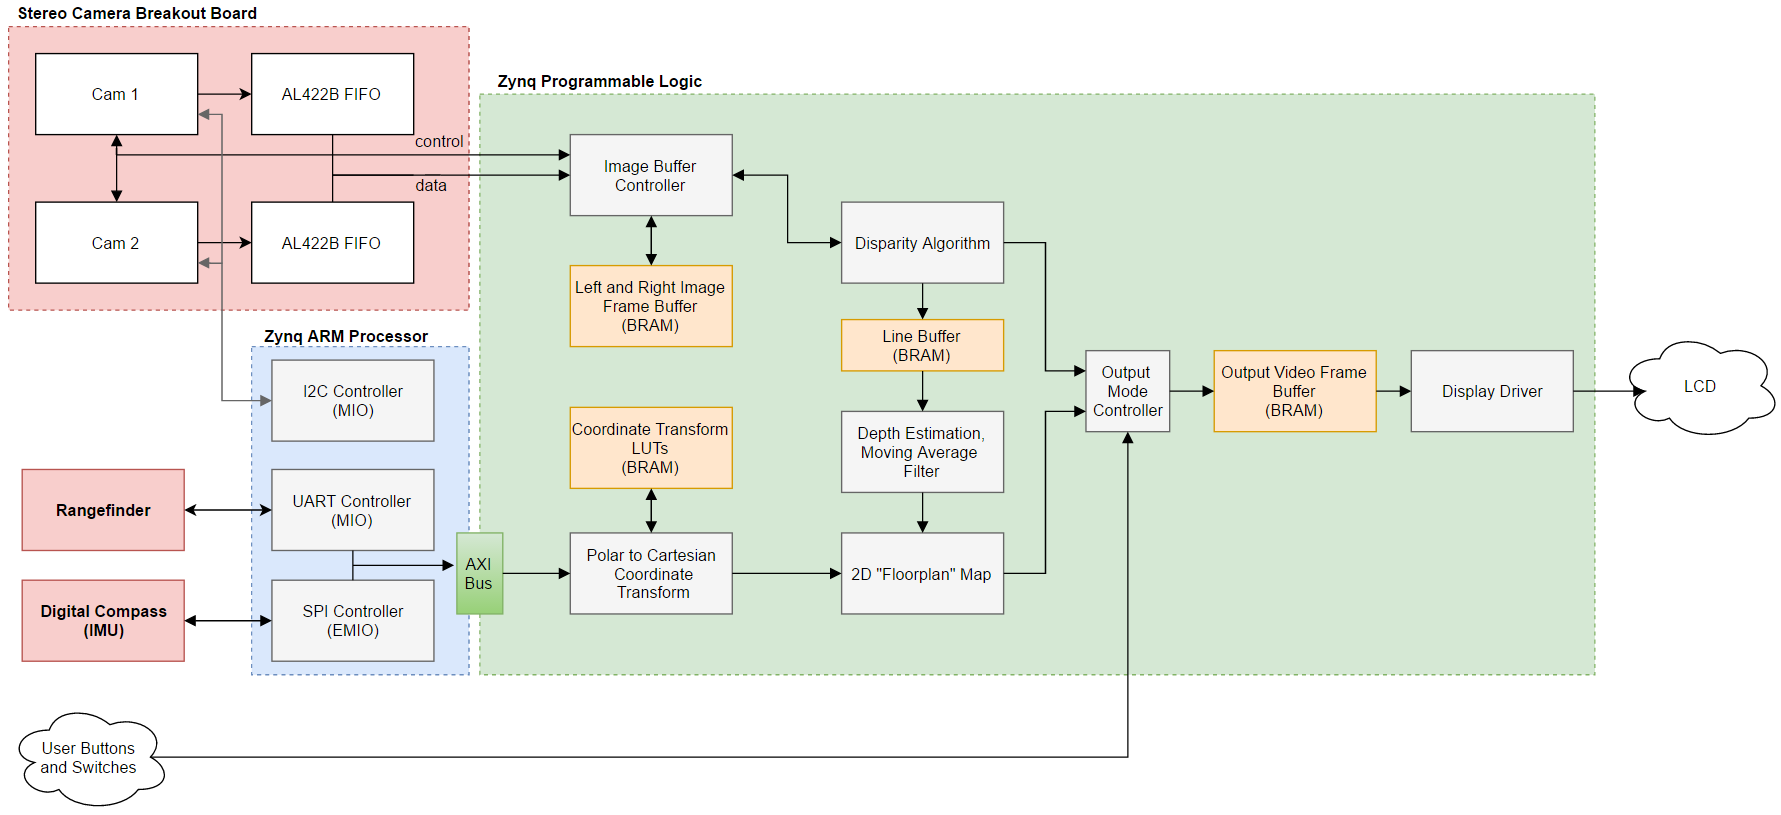
\includegraphics[width=1.25\linewidth]{full_blockdiag.png}
	}
	\caption{Final System Block Diagram}
	\label{systemBD2}
\end{figure}
\par
The programmable logic for this implementation consisted of two main processing pipelines. One main functional process of the PL was to parse image data into depth measurements using disparity. The other was to read rangefinder and digital compass data from the programmable software and convert said data into a compass-referenced 2D "floorplan". Both the stereo disparity and 2D floorplan data paths were then combined at the output stage, allowing for resultant data to be viewed on an attached VGA display based on the current operating mode.
\par
In order to create a fully integrated hardware-software interface that allowed for communication between the Zynq FPGA fabric and ARM processor, a custom AXI IP core was created. This IP core served as a top module for all programmable logic located within the green portion of Figure \ref{systemBD2}. This included all user-defined logic for the rangefinder, digital compass, camera interfaces, and VGA controller.
\par
This implementation supported several output modes based on the positions of the user switches. These output modes include a rangefinder mode, disparity mode, and combined 2D "floorplan" mode. As a demonstration of the device output modes, the sensor suite was used to observe the scene shown in Figure \ref{demoScene}, and each output mode was then documented.
\par
\begin{figure}[H]
	\centerline{
	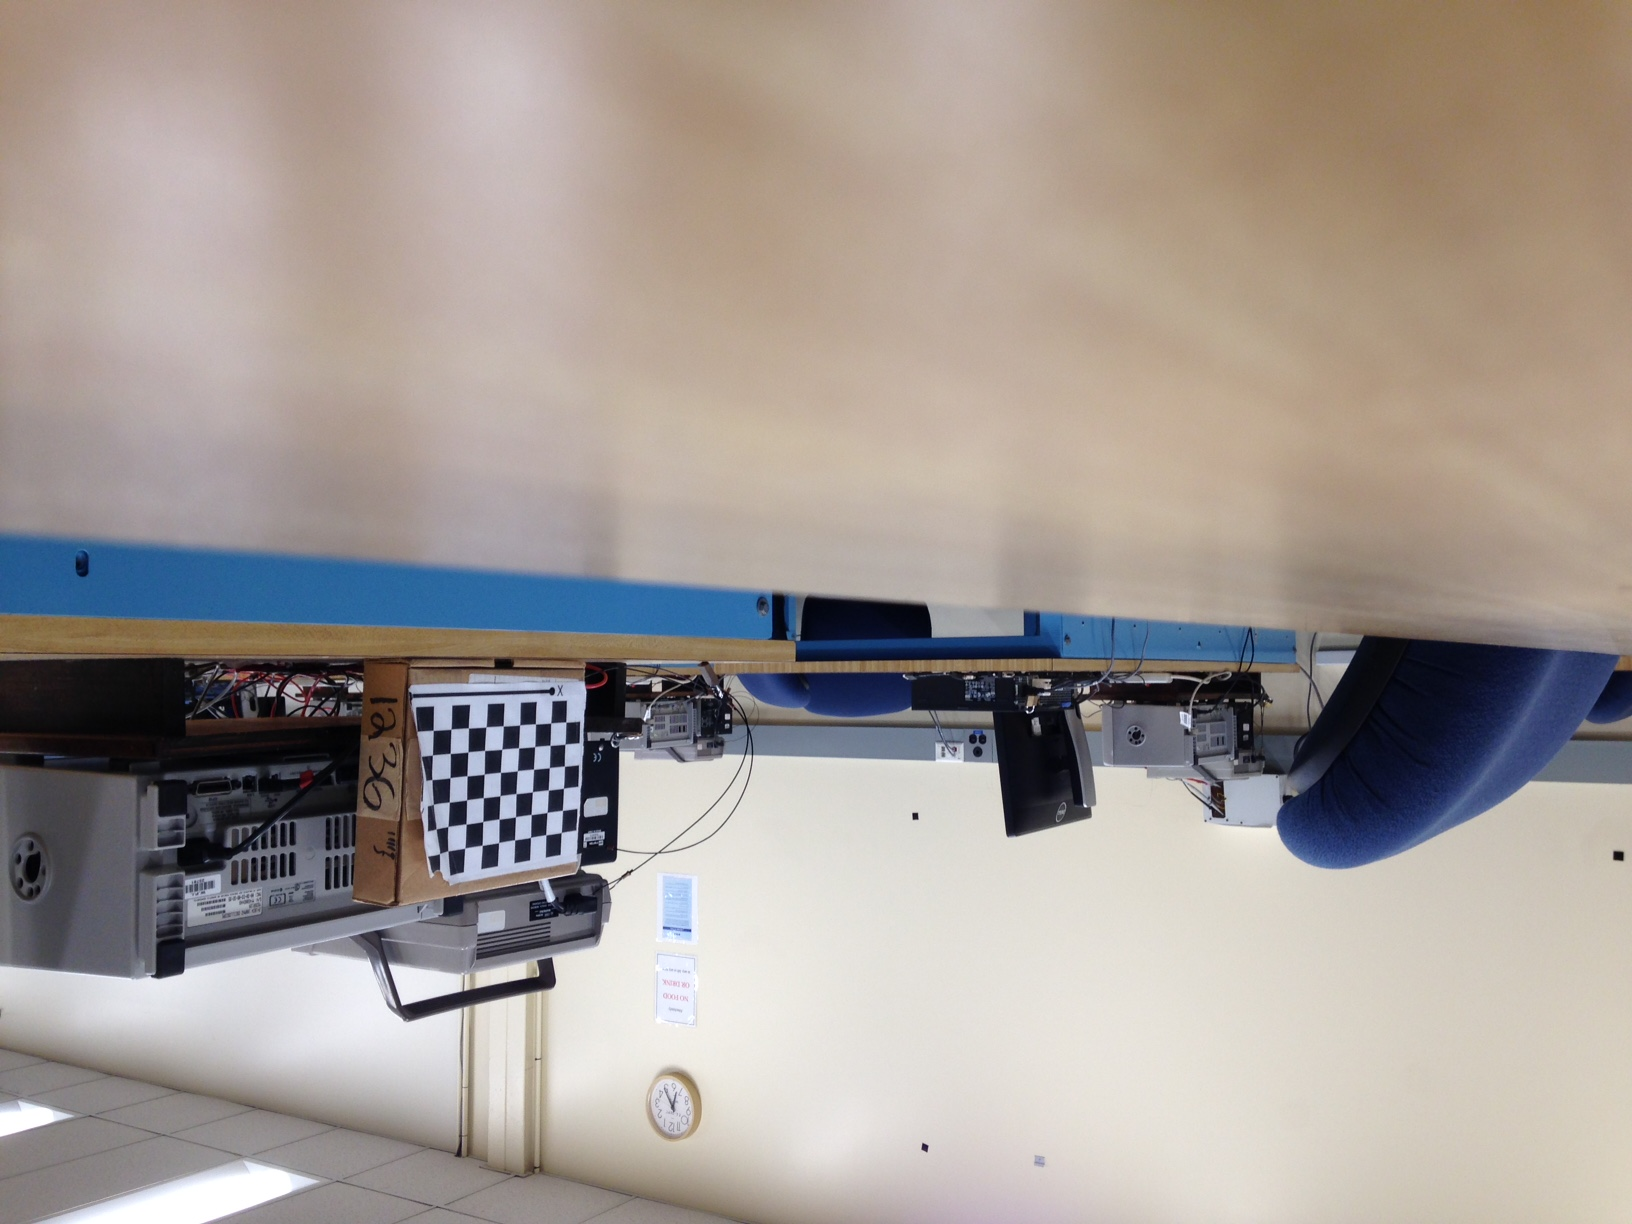
\includegraphics[width=0.6\linewidth]{camera_mode_view.JPG}
	}
	\caption{Demonstration Scene}
	\label{demoScene}
\end{figure}
\par
By default, the system was placed in rangefinder output mode, as shown in Figure \ref{rangeOutputs}a. In this mode, objects found by the scanning laser rangefinder were displayed in black. The entire scan was also localized to the device's central location, shown in red. All rangefinder data was pre-processed by the programmable software to include an offset from the digital compass before being written to programmable logic. In Figure \ref{rangeOutputs}, picture (a) shows the rangefinder output with the device facing due north, while picture (b) shows the rangefinder output with the device rotated west by approximately 90$^\circ$.
\par
\begin{figure}[H]
\centering
       \begin{subfigure}[h]{1\textwidth}
            \centerline{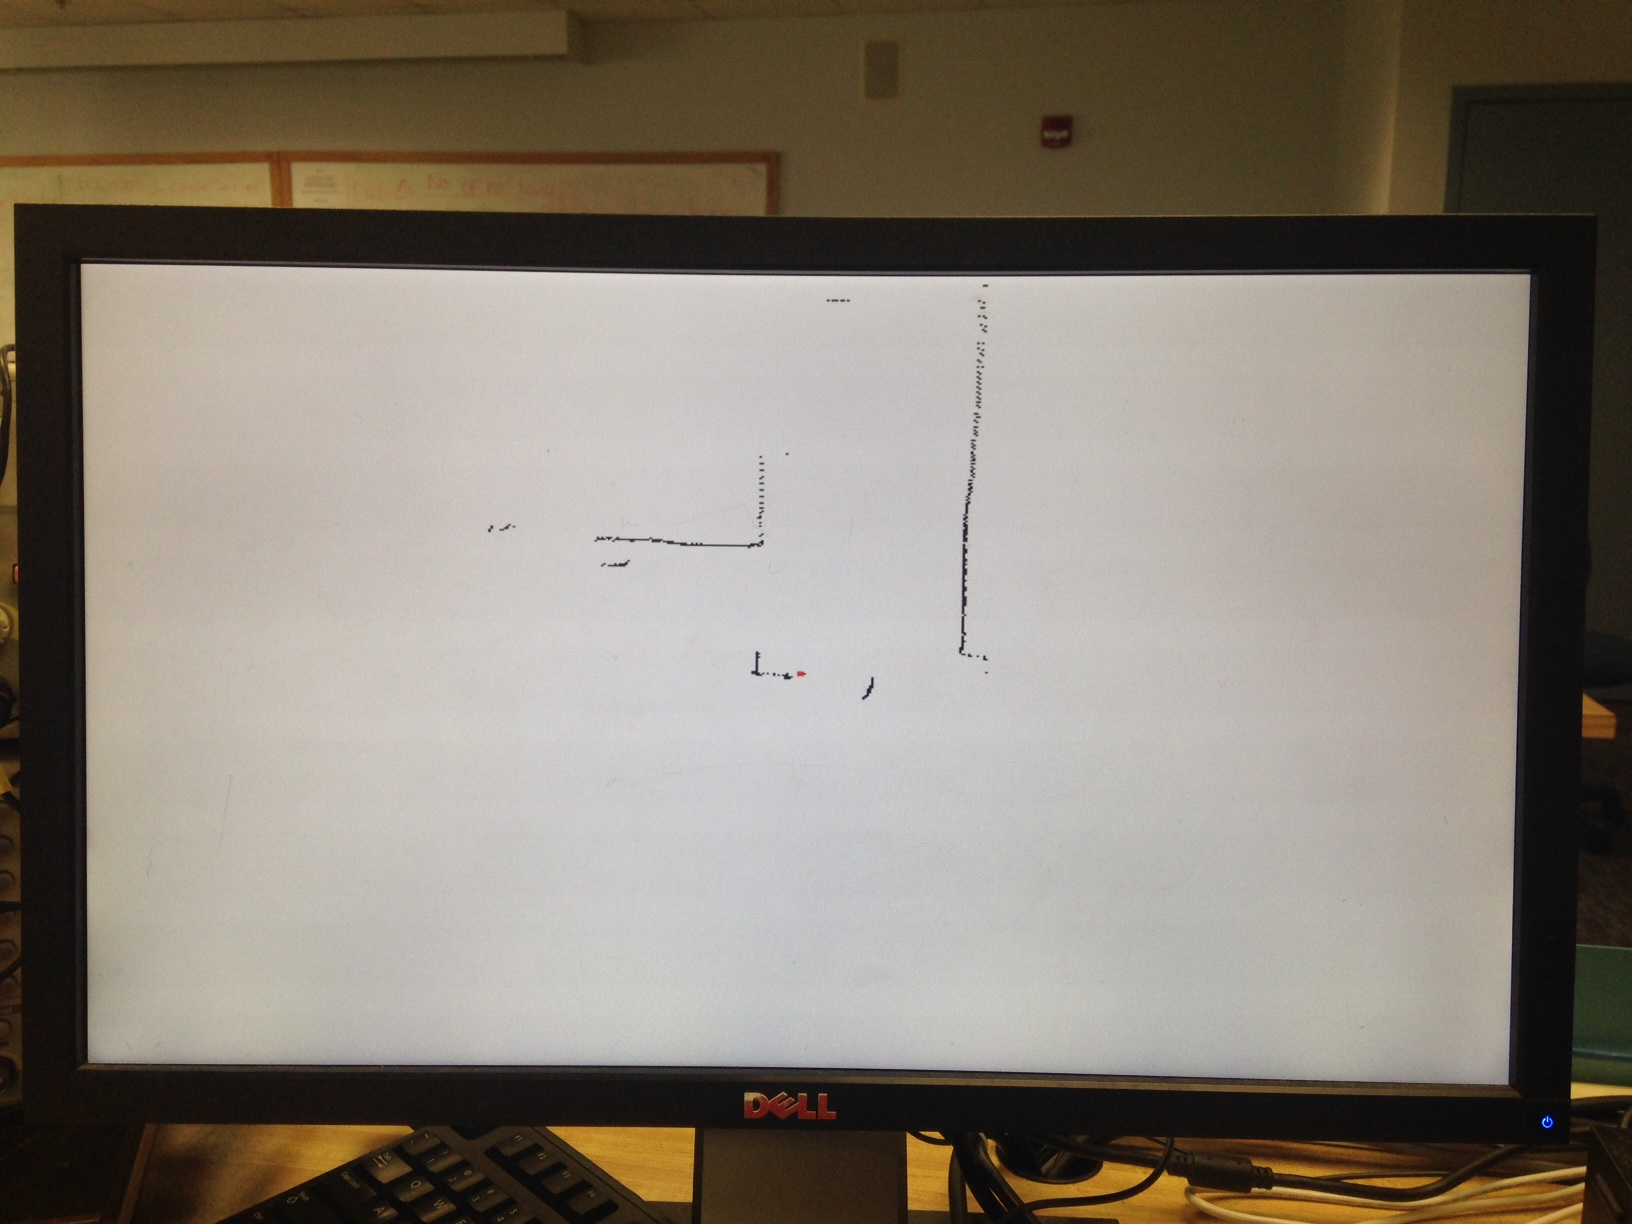
\includegraphics[width=1.0\textwidth]{rangefinder_mode.JPG}}
           \caption{Rangefinder Output}
       \end{subfigure}
       \begin{subfigure}[h]{1\textwidth}
           \centerline{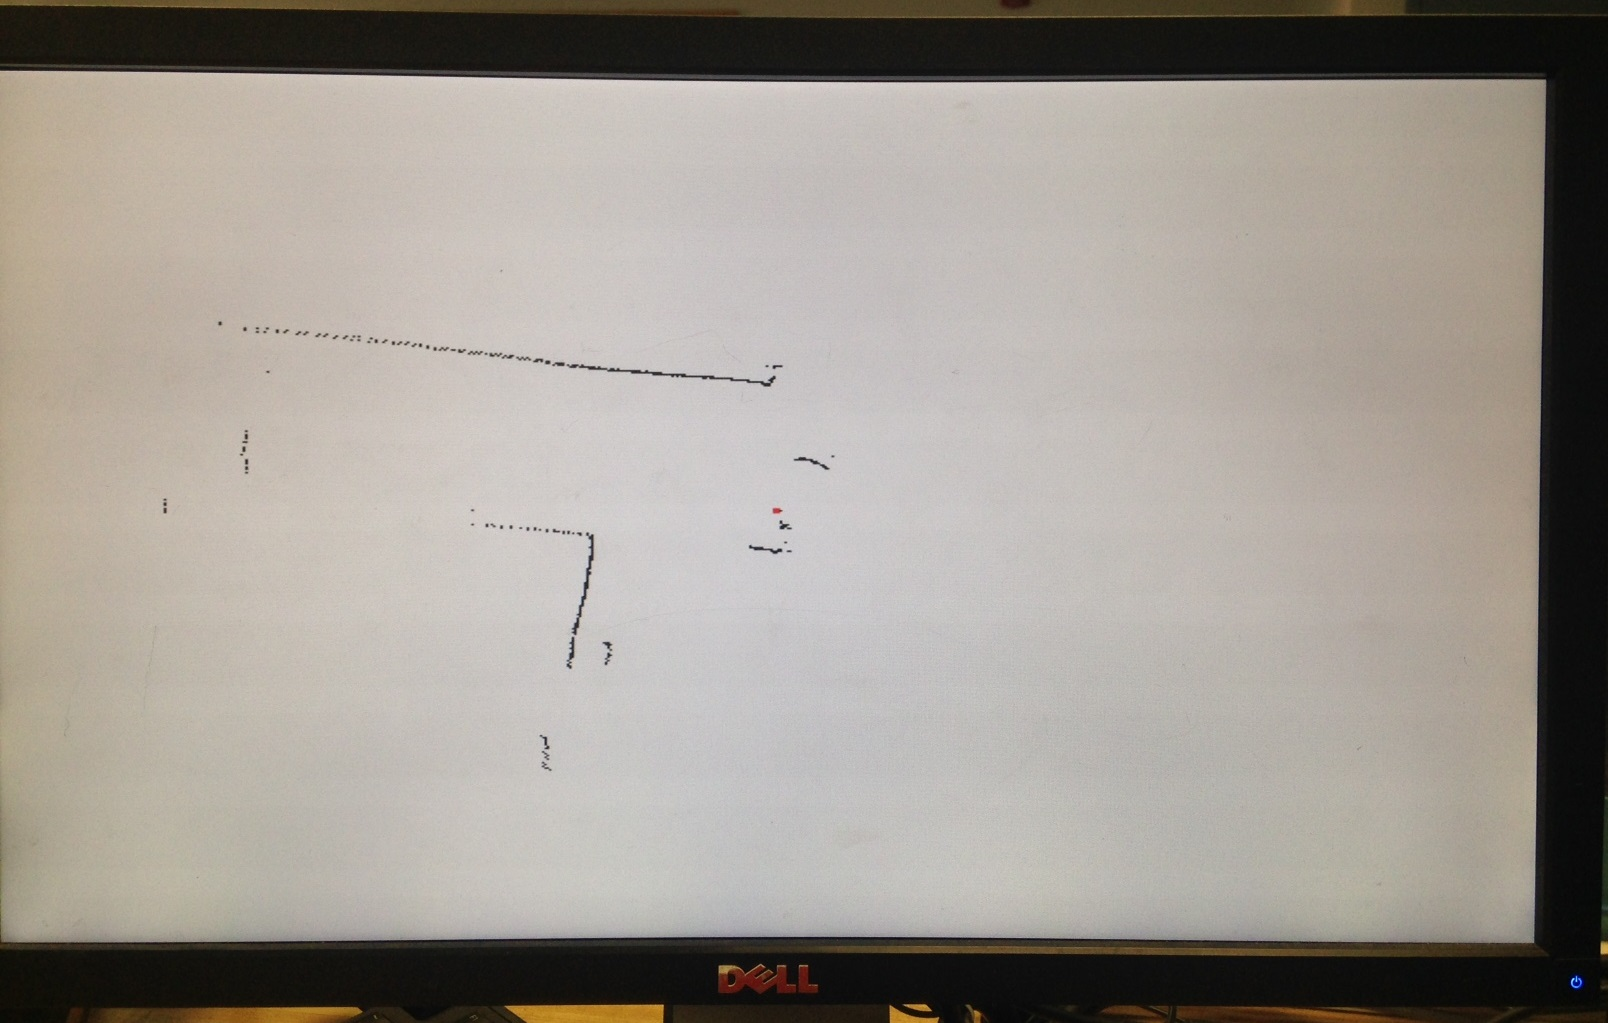
\includegraphics[width=1.0\textwidth]{rangefinder_mode_rotated.JPG}}
           \caption{Rotated Rangefinder Output}
       \end{subfigure}
\caption{2D "Floorplan" Output Modes}
\label{rangeOutputs}
\end{figure}
\par
A second device output mode was included for displaying continuous stereo disparity. While in disparity mode, a 384x288 pixel depth map was continuously updated to reflect the camera's current field of view. An example of the system output for this mode may be found in Figure \ref{disparityOutputs}.
\begin{figure}[H]
        \centerline{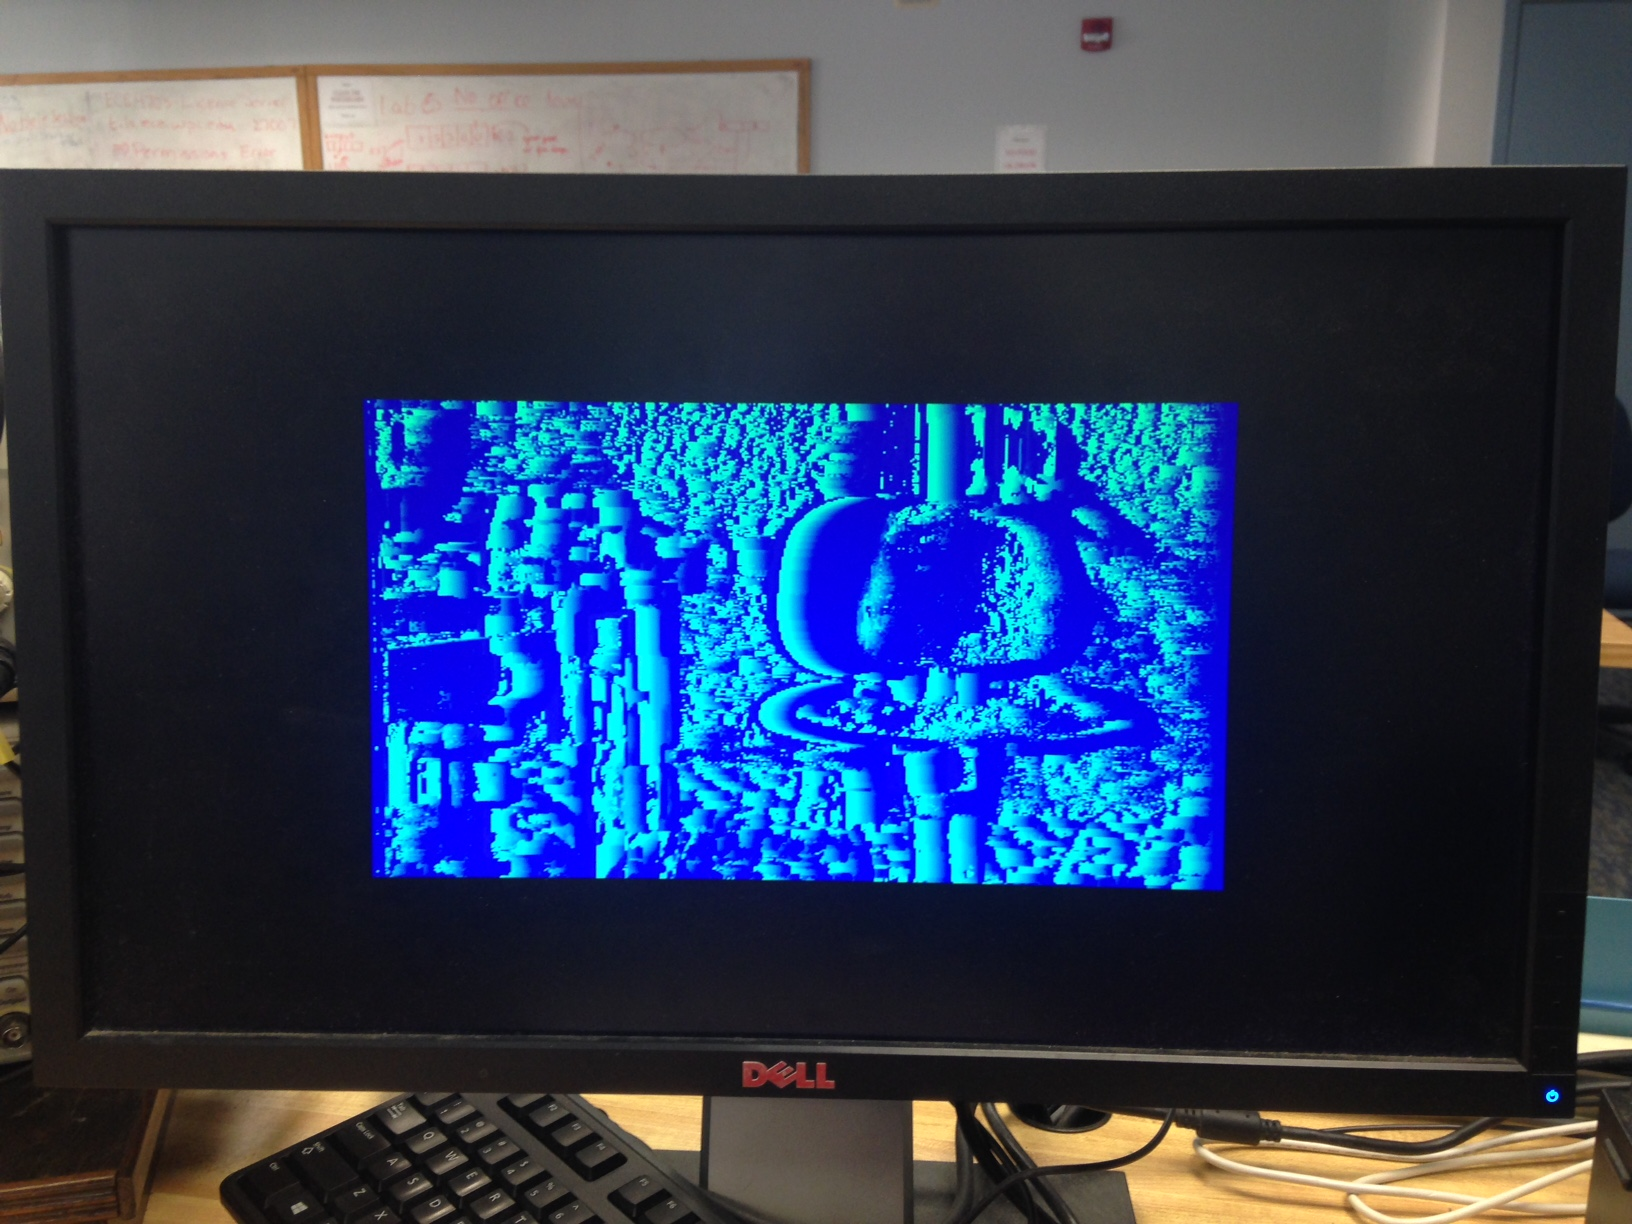
\includegraphics[width=1.0\textwidth]{disparity_mode.JPG}}
        \caption{Disparity Output Mode}
        \label{disparityOutputs}
\end{figure}
\par
A final output mode was also included to incorporate filtered disparity data overlaid onto the 2D "floorplan" produced by the rangefinder. By combining data from both sensors, the stereo cameras were able to account for situations where the scanning laser rangefinder was out of range due to limitations in viewing distance. This output mode is shown in Figure \ref{combinedOut}.
\par
\begin{figure}[H]
	\centerline{
	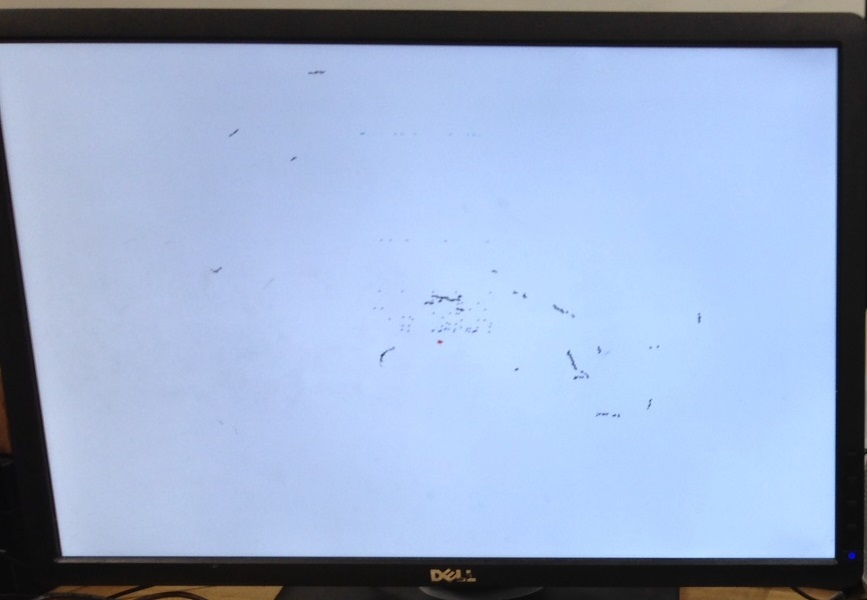
\includegraphics[width=1\linewidth]{combined_mode.JPG}
	}
	\caption{Combined Output Mode}
	\label{combinedOut}
\end{figure}
\par
Several steps were taken during the creation of each output mode to aid in hardware debugging. As a basic confirmation of working hardware, the current state of the rangefinder or disparity state machines were passed to the ZedBoard's LEDs. Another important debugging step included an additional output mode that showed the current camera images being used by the disparity algorithm. An example of this mode's output is shown in Figure \ref{camOutMode}. Note that the image coloration was a result of mapping a monochrome image to arbitrary VGA colors to account for a lack of grayscale color space.
\par
\begin{figure}[H]
	\centerline{
	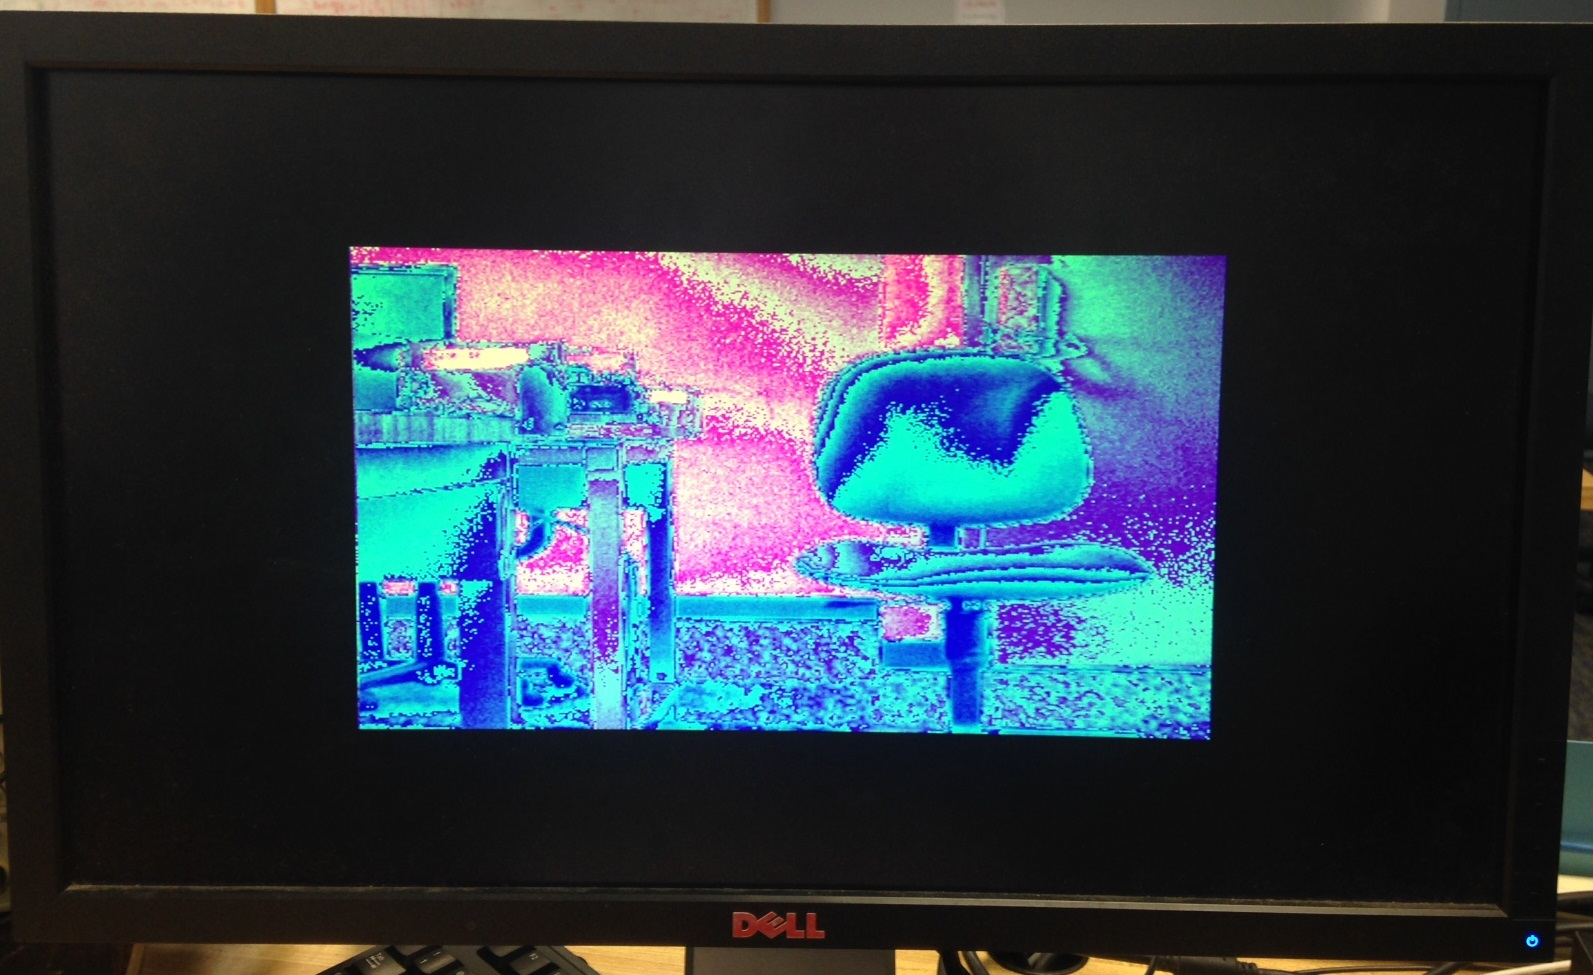
\includegraphics[width=1\linewidth]{camera_mode.JPG}
	}
	\caption{Raw Camera Data Mode}
	\label{camOutMode}
\end{figure}



